\subsection{Rimbalzi}

Guardando lo scatter plot di misure in coincidenza, abbiamo notato dei comportamenti non attesi che abbiamo supposto e poi verificato essere dei fotoni che rimbalzano da un rivelatore all'altro.

La \autoref{scatter} mostra un tipico scatter plot nella configurazione in cui 2 rivelatori sono posti uno di fronte all'altro alla stessa distanza da una sorgente di \na{}.

\begin{figure}[h]
\centering
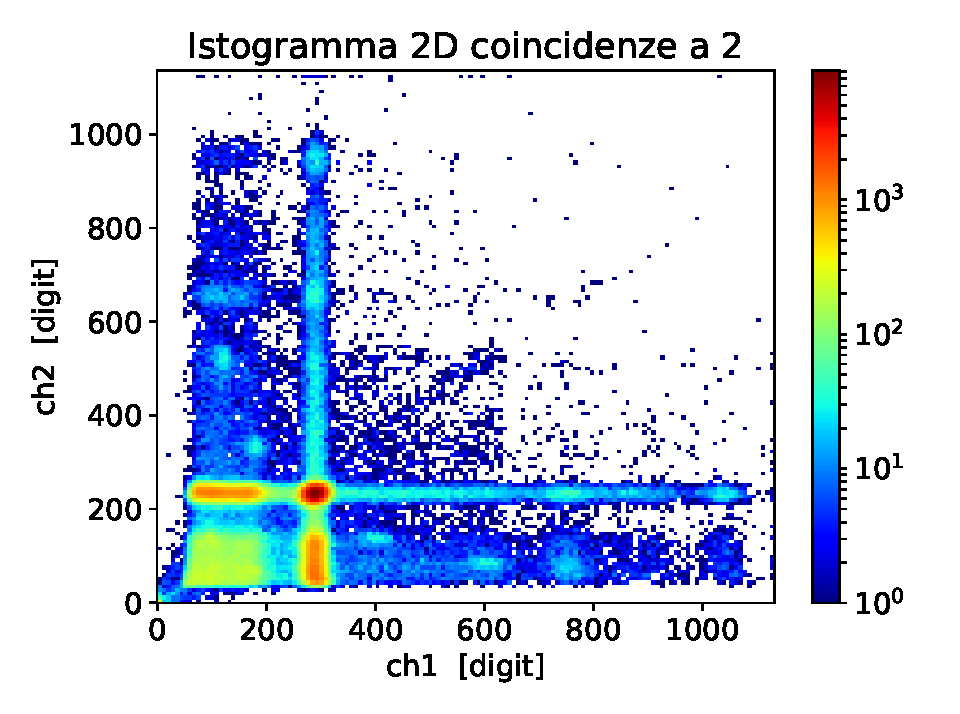
\includegraphics[width=\textwidth]{immagini/esempio}
\caption{Tipico scatter plot di una misura in coincidenza. La descrizione di questo grafico è presente nel testo.}
\label{scatter}
\end{figure}

\marginpar{Chiedere a Jack di fare il super grafico con istogrammi 1D e 2D se non si perde troppo tempo}

Si vedono degli eccessi in alcuni punti del grafico che chiameremo in seguito \emph{strutture}. La più vistosa si manifesta quando entrambi i fotoni di annichilazione effettuano un processo fotoelettrico all'interno degli scintillatori. In basso a sinistra si nota invece la zona in cui entrambi hanno subito una diffusione Compton. Le bande arancioni intorno a questa zona rappresentano invece gli eventi in cui un fotone proveniente dall'annichilazione ha fatto fotoelettrico su un rivelatore e l'altro ha fatto Compton sull'altro.
La stessa cosa avviene con il fotone proveniente dal decadimento del neon, rappresentato dalle strutture nella parte centrale del grafico adiacente ai bordi della figura. La struttura più a destra (o più in alto) rappresenta l'arrivo simultaneo di un fotone di annichilazione insieme ad uno del neon. L'interpretazione degli eventi è analoga a quelli descritti precedentemente.

\marginpar{Non sarebbe male mettere una legenda sui picchi.}

Le strutture non attese sono i due eccessi presenti nella zona in cui il fotone del neon e quello dell'annichilazione fanno entrambi scattering Compton. Queste strutture si manifestano a valori di energia coincidenti ai picchetti della spalla Compton
\marginpar{``Picchetti della spalla Compton'' non è molto chiaro, ma ci penserò più tardi a come aggiustarli.}

Per verificare la nostra ipotesi abbiamo messo i rivelatori nella configurazione di \autoref{spostati}, in modo da poterci aggiungere dei mattoni di piombo come in \autoref{spostati2}. \marginpar{AGGIUSTARE}
Lo scatter plot corrispondente si trova in \autoref{spostato}: la struttura più popolata non è più data dalla rivelazione simultanea dell'annichilazione per effetto fotoelettrico, ma dalla somma degli eventi nelle bande che si incrociano.
In questa configurazione non si nota più uno degli eccessi inattesi nominati prima: quello ad energia più alta. Adesso sono diventate evidenti due strutture circolari nella zona in basso a sinistra del grafico: esse e l'ultimo tipo di struttura rimasta scompaiono completamente quando effettuiamo la misura nella configurazione mostrata in \autoref{spostati2}, come mostrato in \autoref{piombo}.

\begin{figure}[h]
\centering
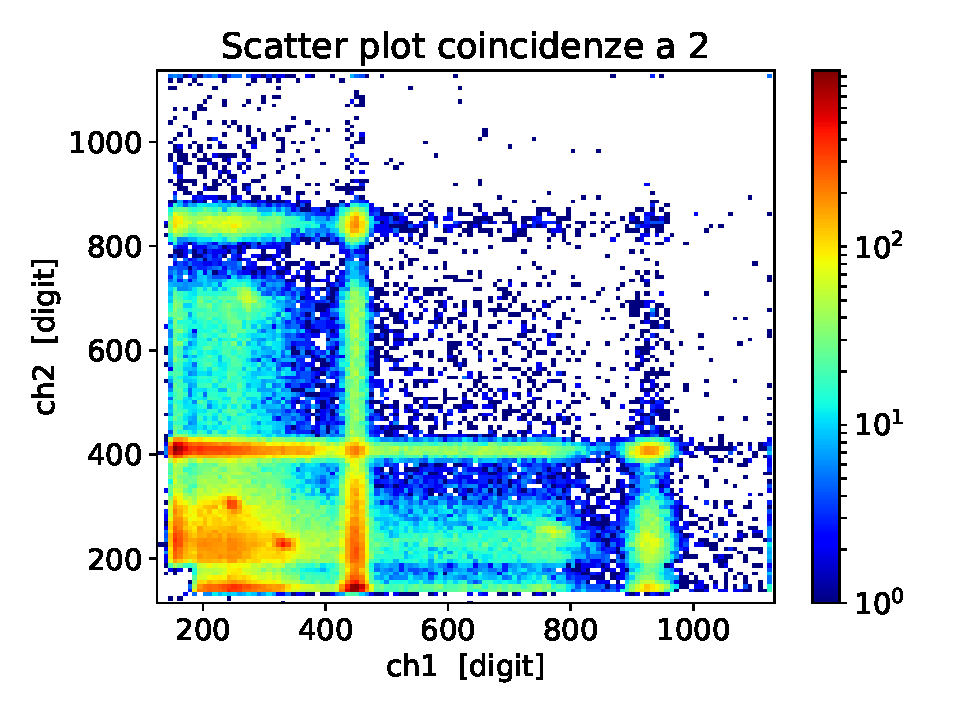
\includegraphics[width=\textwidth]{immagini/0518_rimbalzi}
\caption{Misura eseguita nella configurazione di \autoref{spostati}. La descrizione del grafico è presente nel testo.}
\label{spostato}
\end{figure}

\begin{figure}[h]
\centering
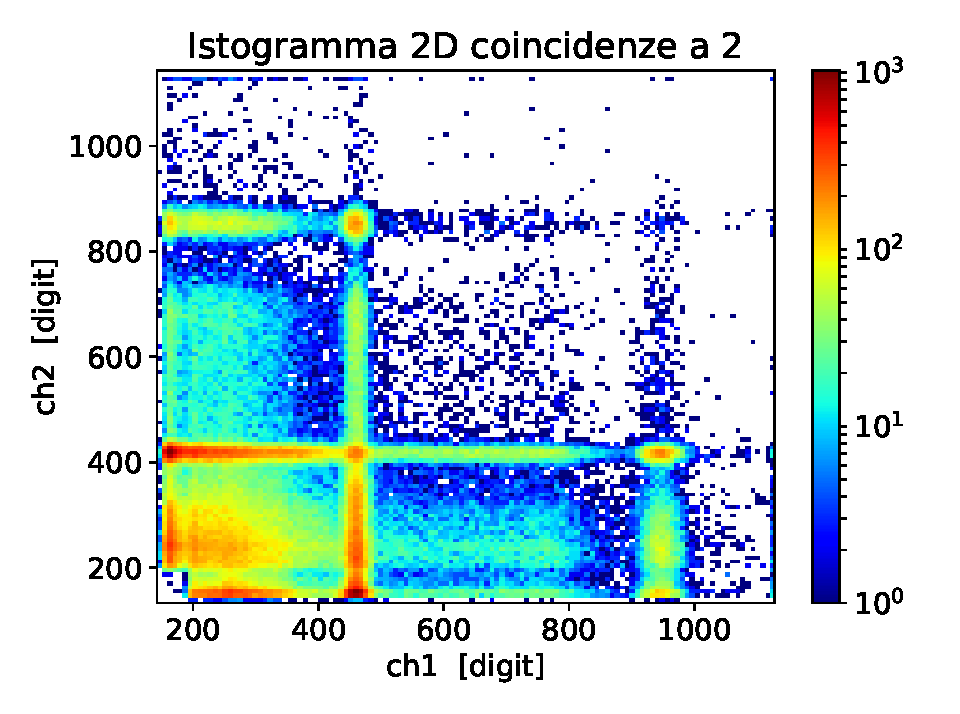
\includegraphics[width=\textwidth]{immagini/0518_piombo}
\caption{Misura eseguita nella configurazione di \autoref{spostati2}. La descrizione di questo grafico è presente nel testo.}
\label{piombo}
\end{figure}


\subsubsection{Misura con un solo fotone}

Abbiamo effettuato la misura nella configurazione di \autoref{solo} e poi \autoref{solo_pb} usando la sorgente di \cs{}: lo scopo della misura è quantificare l'importanza di un rimbalzo tra scintillatori vicini.

 
